%MinLoc

\begin{figure}[h]
	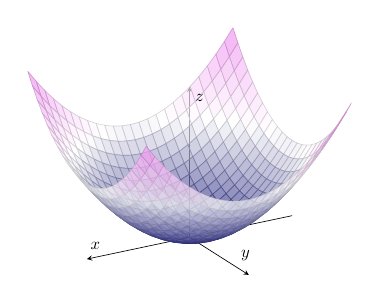
\begin{tikzpicture}[scale=0.6]
		\begin{axis}[view={150}{30}, axis lines=middle, xlabel=$x$, ylabel=$y$, zlabel=$z$,
			ticks=none]
			\addplot3[surf,domain=-1:1,domain y=-1:1,opacity=0.7, colormap/violet] 
			{x^2 + y^2}; % Funzione con un minimo locale in (0,0)
		\end{axis}
	\end{tikzpicture}
\end{figure}